\chapter{The \LHC and \CMS detector}
\label{chap:detector}

%\chapterquote{}{}

%------------------------------------------------------------------------------%
\section{Introduction}

% TODO: Careful of overlap with introduction chapter
The \LHC was built with the design goal of leading the energy frontier of high
energy physics. This led to the successful discovery of the Higgs bosons by the
\ATLAS \cite{Aad:1471031} and \CMS experiments \cite{Chatrchyan:1471016}.
Moreover, \BSM searches with these experiments continue to push stringent
limits on the possible parameter-space of theorised new physics scenarios. Such
discoveries and searches are only possible by the hugely complex detectors
and the \LHC accelerator complex, built and maintained by thousands of Engineers
and Physicists.

%------------------------------------------------------------------------------%
\section{The \LHC}

\subsection{Accelerator Complex}

Proton collisions at the \LHC start from the ionisation of hydrogen gas to
liberate the proton nuclei from their bound atomic states. The protons are
accelerated by the RF-cavity based accelerator \LINACTWO and injected into the
\PSBooster --- four superimposed synchrotron rings accelerating protons from
${\SI{50}{MeV}}$ to ${\SI{1.4}{GeV}}$ --- allowing the injection of more
protons into the \PS. The \PS is a synchrotron with a radius of
${\SI{72}{m}}$ bending the proton beam into a ring with energies up to
${\SI{25}{GeV}}$ before injection into the \SPS. Prior to the injection the
proton beam is bunched into discrete packets of protons about ${\SI{4}{ns}}$
long with an equal spacing of ${\SI{25}{ns}}$ required by the \LHC for a
bunch crossing rate of ${\SI{40}{MHz}}$. The \SPS is another synchrotron
with a larger radius of ${\SI{6.9}{km}}$ to accommodate the acceleration of
protons up to ${\SI{450}{GeV}}$ for the extraction by the \LHC. The whole
accelerator complex allows the \LHC to accelerate protons bunches at energies
of ${\SI{6.5}{TeV}}$ with a bunch crossing period of ${\SI{25}{ns}}$ and
luminosities of the order of ${\SI{e34}{cm^{-2}s^{-1}}}$. The schematic of 
this accelerator complex is shown in Fig.~\ref{fig:LHC-Complex} \cite{Benedikt:823808}.

\begin{figure}[!htbp]
    \centering
    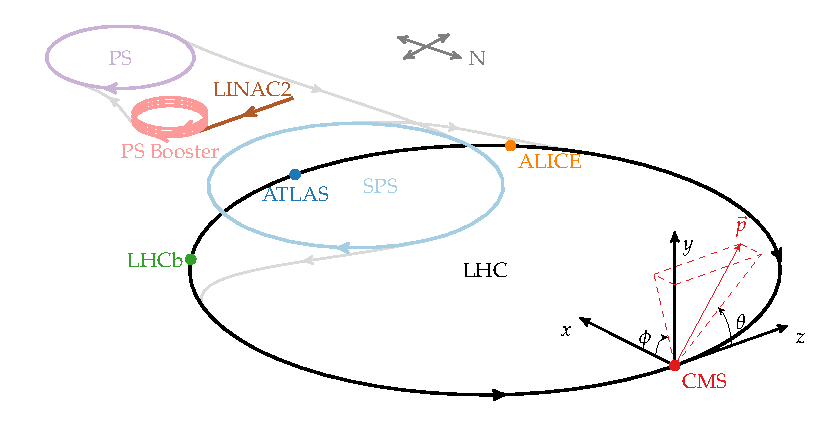
\includegraphics{diagrams/tikz/lhc_complex/lhc_complex.pdf}
    \caption{\cite{Mobs:2197559}}
    \label{fig:LHC-Complex}
\end{figure}

\subsection{\LHC Main Ring}

The main physics goals of the \LHC project was the discovery of the Higgs boson
and to observed new and rare \SM processes. The expected number of event rate of
a particular process with a cross section $\xs$ at a beam luminosity
$L$ is

\begin{equation}
    \mathcal{N} = L \xs \ .
\end{equation}

To increase the event rate the beam luminosity must increased. For Gaussian
beam distributions the luminosity can be given in terms of beam parameters as

\begin{equation}
    \label{eq:beam-lumi}
    L = \frac{N_b^2 n_b\frev\relgamma}{4\pi\emitt\bstar} F\ ,
\end{equation}

where $N_b$ is the number of particles per bunch, $n_b$ is the number of bunches
per beam, \frev is the revolution frequency, \relgamma is the relativistic gamma
factor, \emitt is the normalised transverse beam emittance, \bstar is the beta
function at the collision point (related to the transverse size of the beam) and
$F$ is the geometric luminosity reduction factor due to the crossing angle of
each beam at the crossing point.

At the \LHC, the luminosity is maximised by tuning all parameters in
Eq.~\eqref{eq:beam-lumi}. This necessitated the use of proton beams, circulating
in separate vacuum chambers and merging at insertion points to the detectors.
The beams nominally circulate in 2808 bunches with a spacing of ${\SI{25}{ns}}$
inside twin bore superconducting magnets --- two sets of coils and beam channels
within the same structure and cryostat --- achieving a peak dipole field of
${\SI{8.33}{T}}$ to bend the beam. Radio-frequency (RF) cavities apply the
potential gradient to accelerate the protons from ${\SI{450}{GeV}}$ to
${\SI{6.5}{TeV}}$. Quadrupole magnets focus the beam to suppress dispersion,
hence maintaining the beam luminosity. Additional quadrupoles focus the
beam as they enter the collision sections and defocus as they exit 
\cite{Bruning:782076}.

\section{Compact Muon Solenoid (\CMS) Experiment}

The \CMS detector, centered on one of the \LHC's collision points, is a general
purpose detector with a ${\SI{13}{m}}$ long, ${\SI{5.9}{m}}$ inner diameter,
${\SI{3.8}{T}}$ superconducting solenoid enclosing tracking and calorimetry
subdetectors. An iron return yoke maintains a ${\SI{2}{T}}$ field outside the
solenoid for the muon subdetectors. All subdetectors are segmented into various
regions in $\eta$ known as the barrel (covering the central $\eta$ range) and
endcap (covering up to $\aeta=3$ with some overlap with the barrel). The
hadronic calorimeter has an additional segment in the forward region (covering
$3<\aeta<5$) to extend the coverage of hadronic activity. Further subdetector
dependent segmentation is done within the barrel, endcap and forward regions.
This gives \CMS the total length of ${\SI{21.6}{m}}$ and diameter of
${\SI{14.6}{m}}$ weighing ${\SI{12500}{tons}}$.

The conditions provided by the \LHC during 2016 data taking resulted in an
average number of collisions per bunch crossing of approximately 20, leading
to 1000 charged particles every ${\SI{25}{ns}}$ bunch crossing. The
subdetectors were designed to account for particle multiplicities of this order
by focusing on high-granularity detectors with good time resolution. This
requires a large number of detector channels and millions of synchronised
detector electronics, all with a high radiation tolerance.

\subsection{Silicon Tracker}

The silicon tracker, the inner most subdetector, uses silicon technology with
reverse-biased p-n junctions to measure positional coordinates of charged
particles. As an ionising particle travels through the junction an electron-hole
pair is created which drift in the electron field towards the cathode or anode.
This signal is amplified and digitised and later used to reconstruct the whole
event as required. The choice of silicon allows for a very granular detector
required to distinguish tracks from the primary, secondary or pileup vertices.

The tracker is ${\SI{5.8}{m}}$ long and ${\SI{2.6}{m}}$ in diameter with 10
layers of silicon microstrip detectors and an additional 3 layers of silicon
pixels near the interaction region for improved measurements of the impacts
parameter of charged particles and position of secondary vertices. The tracker
covers a region of up to ${\aeta=2.5}$.

\subsection{\ECAL}

The \ECAL is a homogeneous calorimeter made of lead tungstate (\pbwo) crystals
designed to provided calorimetric measurements of electromagnetic deposits
(typically electrons and photons) up to ${\aeta=3.0}$. The crystals have
short radiation lengths (${\SI{0.89}{cm}}$) and Moliere lengths
(${\SI{2.2}{cm}}$) allowing a compact design which absorbs a significant
portion of electromagnetic energy with a satisfactory level of radiation
resistance. The low light yield (${\SI{30}{photon/MeV}}$) from the crystals are
detected by photodetectors with intrinsic gain operable in the magnetic field.
Silicon avalanche photodiodes are used in the barrel and vacuum phototriodes in
the endcaps. Along with the barrel and endcaps, the \ECAL has a preshower system
installed in front of the endcaps for ${\Ppizero}$ rejection (since about
${98.8\%}$ of ${\Ppizero}$ decays into two photons with a very short lifetime,
${c\tau=\SI{25.5}{nm}}$). The preshower consists of two planes of silicon strip
detectors behind disks of lead absorber at depths of 2 and 3 radiation lengths.
The barrel covers a range of up to ${\aeta=1.479}$ with crystals of
${\SI{0.0174}{rad}}$ in \dphi and \deta and a length of ${\SI{230}{mm}}$ for
$25.8$ radiation lengths. The endcaps cover the region ${1.479<\aeta<3.0}$ in
an $x$-$y$ grid with a front cross section of ${28.6\times\SI{28.6}{mm^2}}$ and
a length of ${\SI{220}{mm}}$ (24.7 radiation lengths).

The energy resolution of the \ECAL is parameterised by

\begin{equation}
    \left(\frac{\sigma}{E}\right)^{2} = \left(\frac{S}{\sqrt{E}} \right)^{2}
    + \left( \frac{N}{E} \right)^{2} + C^2\ ,
\end{equation}

where $S$ is a stochastic tern, $N$ is a noise term and $C$ a constant term.
The total energy resolution ranges between ${1.50--0.35\%}$ for
${10--\SI{250}{GeV}}$, beyond which the constant term dominates.

\subsection{\HCAL}

The \HCAL is designed to provide calorimetric measurements of hadronic activity
in an event. The barrel and endcap sections consist of brass/scintillator
sampling hadron calorimeters with coverage up to ${\aeta=3}$.

\begin{itemize}
    \item Brass/scintillator sampling hadron calorimeter with coverage up to
        ${\aeta=3.0}$. Scintillation detected by wavelength-shifting fibres
        embedded in the scintillator tiles and channeled to photodetectors
        via clear fibres. Then detected by hybrid photodetectors the provide
        gain and operate in high axial magnetic fields. Outer calorimeter
        in the iron return yoke beyond the magnet covering the barrel region
        adds about three interaction lengths ontop of the 8 provided by the
        inner calorimeter.
    \item Coverage up to ${\aeta=5.0}$ provided by iron/quartz-fibre
        calorimeter. Cerenkov light emitted by the quartz fibres is detected by
        photomultiplers. Ensure full coverage for the measurement of the
        transverse energy of an event.
\end{itemize}

\subsection{Solenoid Magnet}

\begin{itemize}
    \item High-purity aluminium-stabilised conductor and indirect cooling (by
        thermosyphon).
    \item Bending power is designed around measuring muon momenta to a
        resolution of ${\Delta\mom/\mom\approx 10\%}$ at ${\mom = \SI{1}{TeV}}$.
    \item Favourable length/radius ratio chosen to ensure good momentum
        resolution in the forward region.
\end{itemize}

\subsection{Muon Chambers}

\begin{itemize}
    \item Resolution limited by multiple scattering in the central material
        up to $\pt=\SI{200}{GeV}$, when the chamber spatial resolution starts
        to dominate.
    \item Three types of gaseous deetctors.
    \item Barrel region (${\aeta<1.2}$), with low neutron induced background,
        the muon rate is low and residual field is low, drift tube chambers are
        used.
    \item 250 DT chambers in 4 layers. Staggered chambers allow high-\pt muons
        near boundaries to cross at least 3 out of the 4 layers. Each station is
        designed to give $\phi$ precision better and ${\SI{100}{\micro m}}$ in
        position and approximately ${\SI{1}{\milli rad}}$ in direction.
    \item The 2 endcaps, high muon and neutron induced background rate is high,
        and large field, cathode strip chambers are used to cover up to
        ${{\aeta}=2.4}$.
    \item 468 CSCs in 2 endcaps. Trapezoidal shape consisting of 6 gas gaps,
        each gap having radial cathode strips and a plane of anode wires running
        perpendicular to the strips. CSCs are overlapped in phi to avoid gaps
        in muon acceptance. Gas ionization and subsequent electron avalanche
        caused by charged particles produces a charge on the anode and image
        charge on the cathode. Precise precision measurement is made by
        determining the centre-of-gravity of the charge distribution induced on
        the cathode strips. Spatial resolution provided by each chamber from the
        strips is typically ${\SIrange{100}{200}{\micro m}}$ with an angular
        resolution in $\phi$ of the order of ${\SI{10}{\milli rad}}$.
    \item Resistive plate chambers are used in both regions. Operating
        in avalanche mode for good operation at high rates. Good timing
        resolution with coarse position resolution to identify the correct
        bunch crossing. Coverage up to ${\aeta<1.6}$ or ${\aeta<2.4}$.
\end{itemize}

    \begin{itemize}
        \item CMS 2006 detector TDR: \cite{Bayatian:922757}.
        \item CMS 2007 physics TDR: \cite{Bayatian:942733}.
        \item CMS 2005 computing TDR: \cite{Bayatyan:838359}.
        \item CMS 2000 TriDAS TDR: \cite{Bayatyan:706847}.
        \item CMS 2013 L1 trigger upgrade TDR: \cite{Tapper:1556311}.
        \item CMS 2012 HCAL upgrade TDR: \cite{Mans:1481837}.
        \item Luminosity report by CMS: \cite{CMS-PAS-LUM-17-001}.
    \end{itemize}

\subsection{Hardware Trigger}

\subsection{Software Trigger}

\subsection{Worldwide \LHC Computing Grid (\WLCG)}

%------------------------------------------------------------------------------%
